\section{Simulation}
\label{sec:simulation}

\par In this section, a briet description of the circuit modeled through NGspice is going to be presented and the values obtained on it are going to be compared with the ones obtained on octave. The purpose of the simulation was to maximise the merit obtained and, as such, to obtain the values of the gain, bandwidth and the lower and higher  cut off frequencies as well as the input and output impedances.

\par In order to do that, the circuit in study was modelled in the program. For that, transistors of the given models (NPN transistor for the gain stage and PNP transistor for the output stage) were used on the two common amplifiers and the rest of the components specifications changed to be on par with the values optimised through the Matlab software (Simulink) and as seen in the octave sript.

\par With the circuit described, the next step was to analyse the simulations with the introduced values. The first step was to verify if the transistors were functioning in the foward active region, F.A.R mode. To do that the potential difference between the collector and the emitter and the base, for the NPN transistor, were calculated and, for the PNP transistor, the potential difference between the emitter and the collector and the base were calculated. In order to guarantee the previous condition it is necessary to guarantee the following conditions: $V_{CE}>V_{BE}$ and $V_{EC}>V_{EB}$. The results obtained are now presented:

\begin{table}[ht]
  \centering
  \begin{tabular}{|l|r|}
    \hline    
   Vce & 4.92668 V\\ \hline
Vbe & 0.654762 V\\ \hline
Correct F.A.R\\ \hline

     \end{tabular}
  \caption{Confirmation of NPN in FAR mode}
 
\end{table}


\begin{table}[ht]
  \centering
  \begin{tabular}{|l|r|}
    \hline    
   Vec & 5.77796 V\\ \hline
Veb & 0.70695 V\\ \hline
Correct F.A.R\\ \hline

     \end{tabular}
  \caption{Confirmation of NPN in FAR mode}
    
\end{table}

\par The next step was to simulate the operating point, since the values of this simulation are important to determine the incremental parameters. The values are shown in the next table.

\begin{table}[ht]
  \centering
  \begin{tabular}{|l|r|}
    \hline    
   @cb[i] & 0.000000e+00\\ \hline
@ce[i] & 0.000000e+00\\ \hline
@q1[ib] & 7.022567e-05\\ \hline
@q1[ic] & 1.404513e-02\\ \hline
@q1[ie] & -1.41154e-02\\ \hline
@q1[is] & 5.765392e-12\\ \hline
@rc[i] & 1.411536e-02\\ \hline
@re[i] & 1.411536e-02\\ \hline
@rf[i] & 7.022567e-05\\ \hline
@rs[i] & 0.000000e+00\\ \hline
v(1) & 0.000000e+00\\ \hline
v(2) & 0.000000e+00\\ \hline
base & 2.254108e+00\\ \hline
coll & 5.765392e+00\\ \hline
emit & 1.411536e+00\\ \hline
vcc & 1.000000e+01\\ \hline

     \end{tabular}
  \caption{Confirmation of NPN in FAR mode}
  \label{tab:op}
    
\end{table}

\par The rest of the values in study (gain, lower and higher cutoff frequencies and bandwidth),  are presented in the following table. These were obtained using the fuction $meas$ as seen in the NGspice script, taking into account that the gain is the maximum of the voltage output, the cutoff frequencies are the frequencies for which the output voltage is 3db less than the gain (as per definition) and the bandwidth is the difference between those frequencies.

\begin{table}[ht]
  \centering
  \begin{tabular}{|l|r|}
    \hline    
   V Gain&34.1403\\ \hline
Bandwidth&1.22339E+06 Hz\\ \hline
Lower Cut Off Freq& 15.8089 Hz\\ \hline
Higher Cut Off Freq& 1.22341E+06 Hz\\ \hline

    \end{tabular}
  \caption{Gain, cutoff frequencies and bandwidth values}
    \label{tab:results}
\end{table}

\par Next, it is important to understand the purpose of certain elements of the circuit: the coupling capacitors; bypass capacitor and the resistor $R_C$. 

\subsection{Effect of the Coupling Capacitors}

\par The coupling capacitors associated to the respective transistors have the primary function of blocking the DC signal. In fact, taking into account the impedance of a capacitor, when $\omega=0$, $Z_C=\inf$ and the circuit is opened. This is necessary because of the main purpose of an amplifier: amplify the input AC signal. As seen on the classes, through the expression of the lower cutoff frequency, the higher the capacitances, the larger the bandwidth is going to be. As for the higher cutoff frequency little effects are going to be felt with the change of capacitance as shown in the formulae presented by the professor. However, only this tension would imply that the transitor wasn't always in the FAR. As such, an aditional DC independent voltage source is used in order to force it to be always in the required FAR. This DC component is eventually eliminated when the current reaches the other capacitor. All of this helps maintaing the operating point of the transistor, allowing it to operate at lower frequencies.

\subsection{Effect of the Bypass Capacitors}

\par As seen in the lectures, the resistor $R_E$ has the function of lessening the effect of the temperaturre in the DC voltage. However by adding a resistor, the gain will lower. In order to negate this, a capacitor is added in parallel to the resistance. With this, the DC current will be affected by the resistor whilst the AC current passes through the capacitor because of its medium - high frequency (and as such the impedance of the capacitor is small - short circuit).

\subsection{Effect of the Resistor $R_C$}

\par Finally, the effect of $R_C$ on the circuit gain is important to be studied. As the gain is proportional to the value of $R_C$, the higher $R_C$ is, the higher the gain will be and thus the merit. 

\par All of the effects mentioned above can be seen through the graphics below, where it is possible to see the bandwidth, the gain and the lower and higher cutoff frequencies.

\begin{figure}[ht]
\centering
\begin{subfigure}{.5\textwidth}
  \centering
  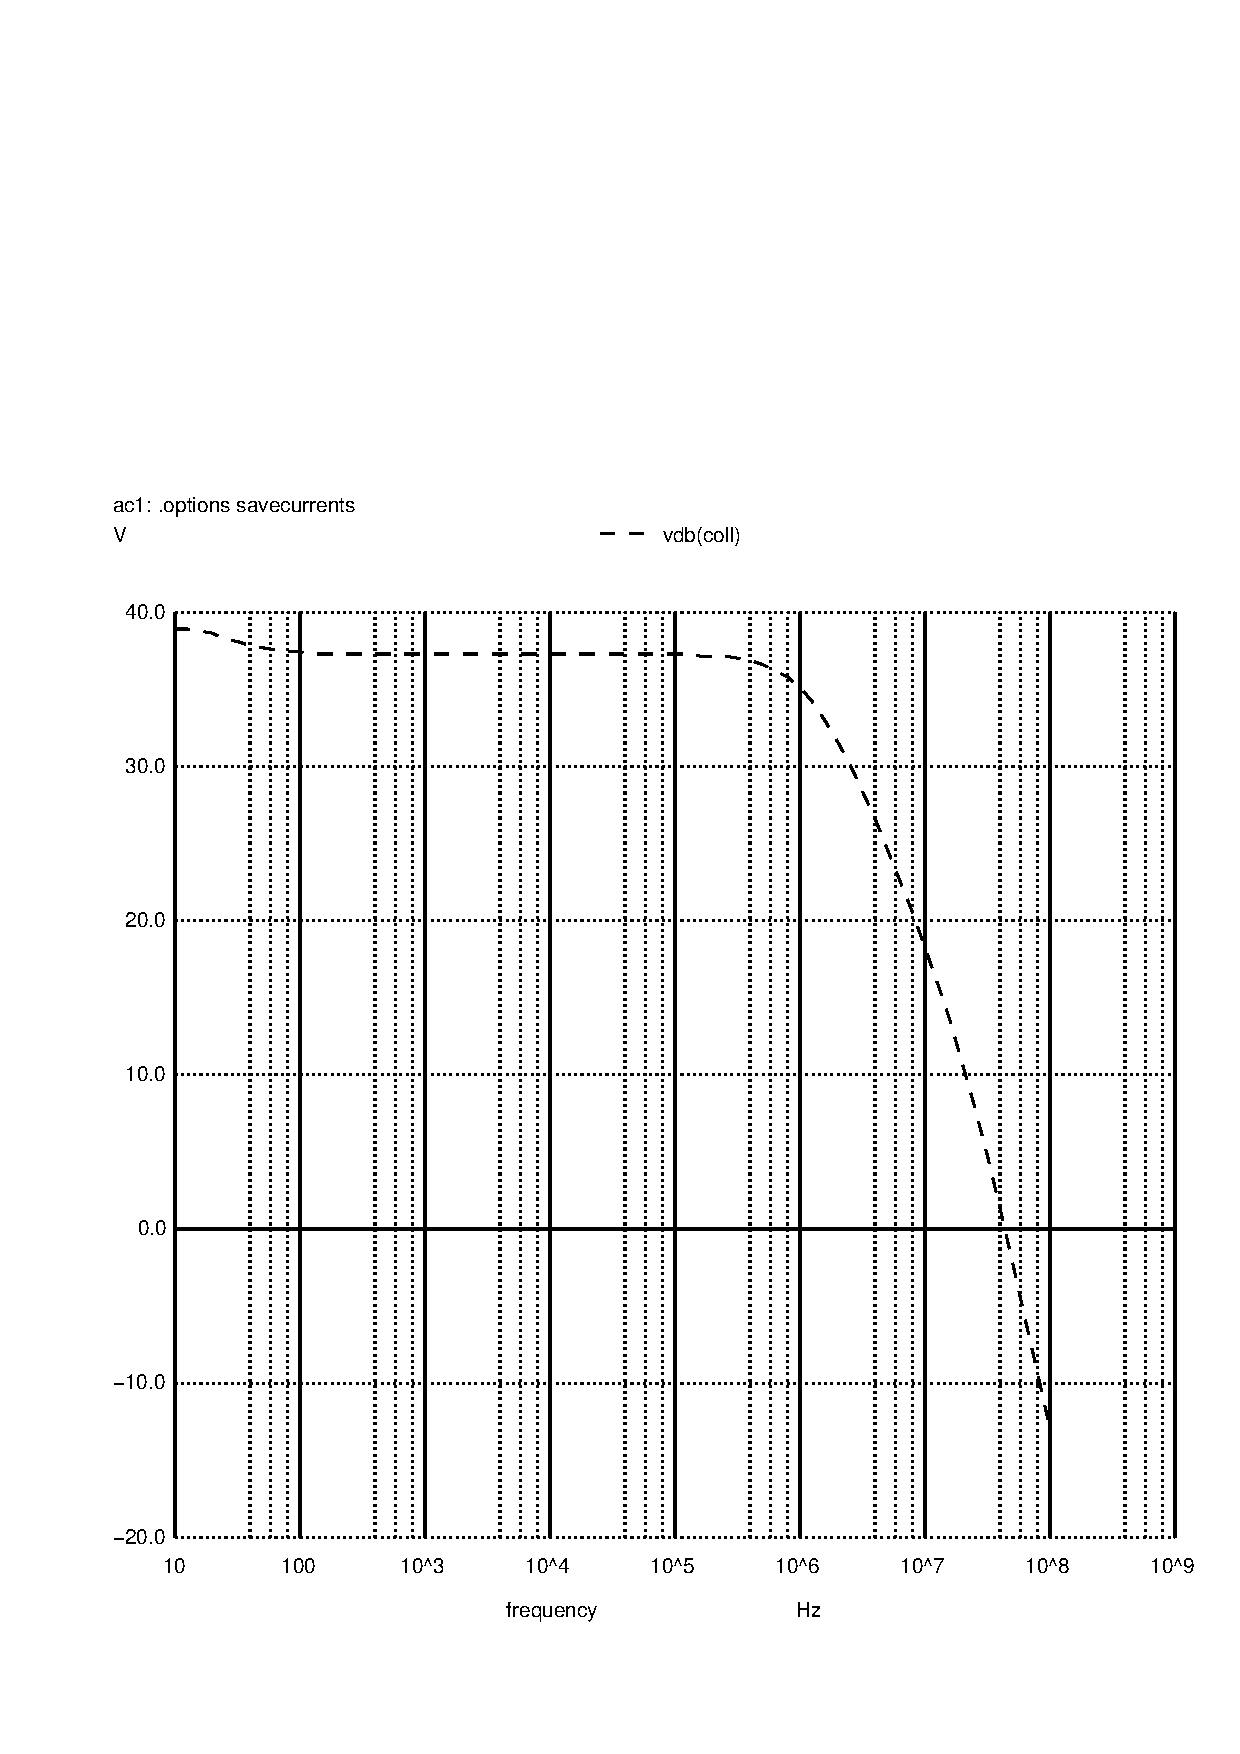
\includegraphics[width=.75\linewidth]{vo1f.pdf}
  \caption{Input Voltage}
  \label{fig:sim4}
\end{subfigure}%
\begin{subfigure}{.5\textwidth}
  \centering
  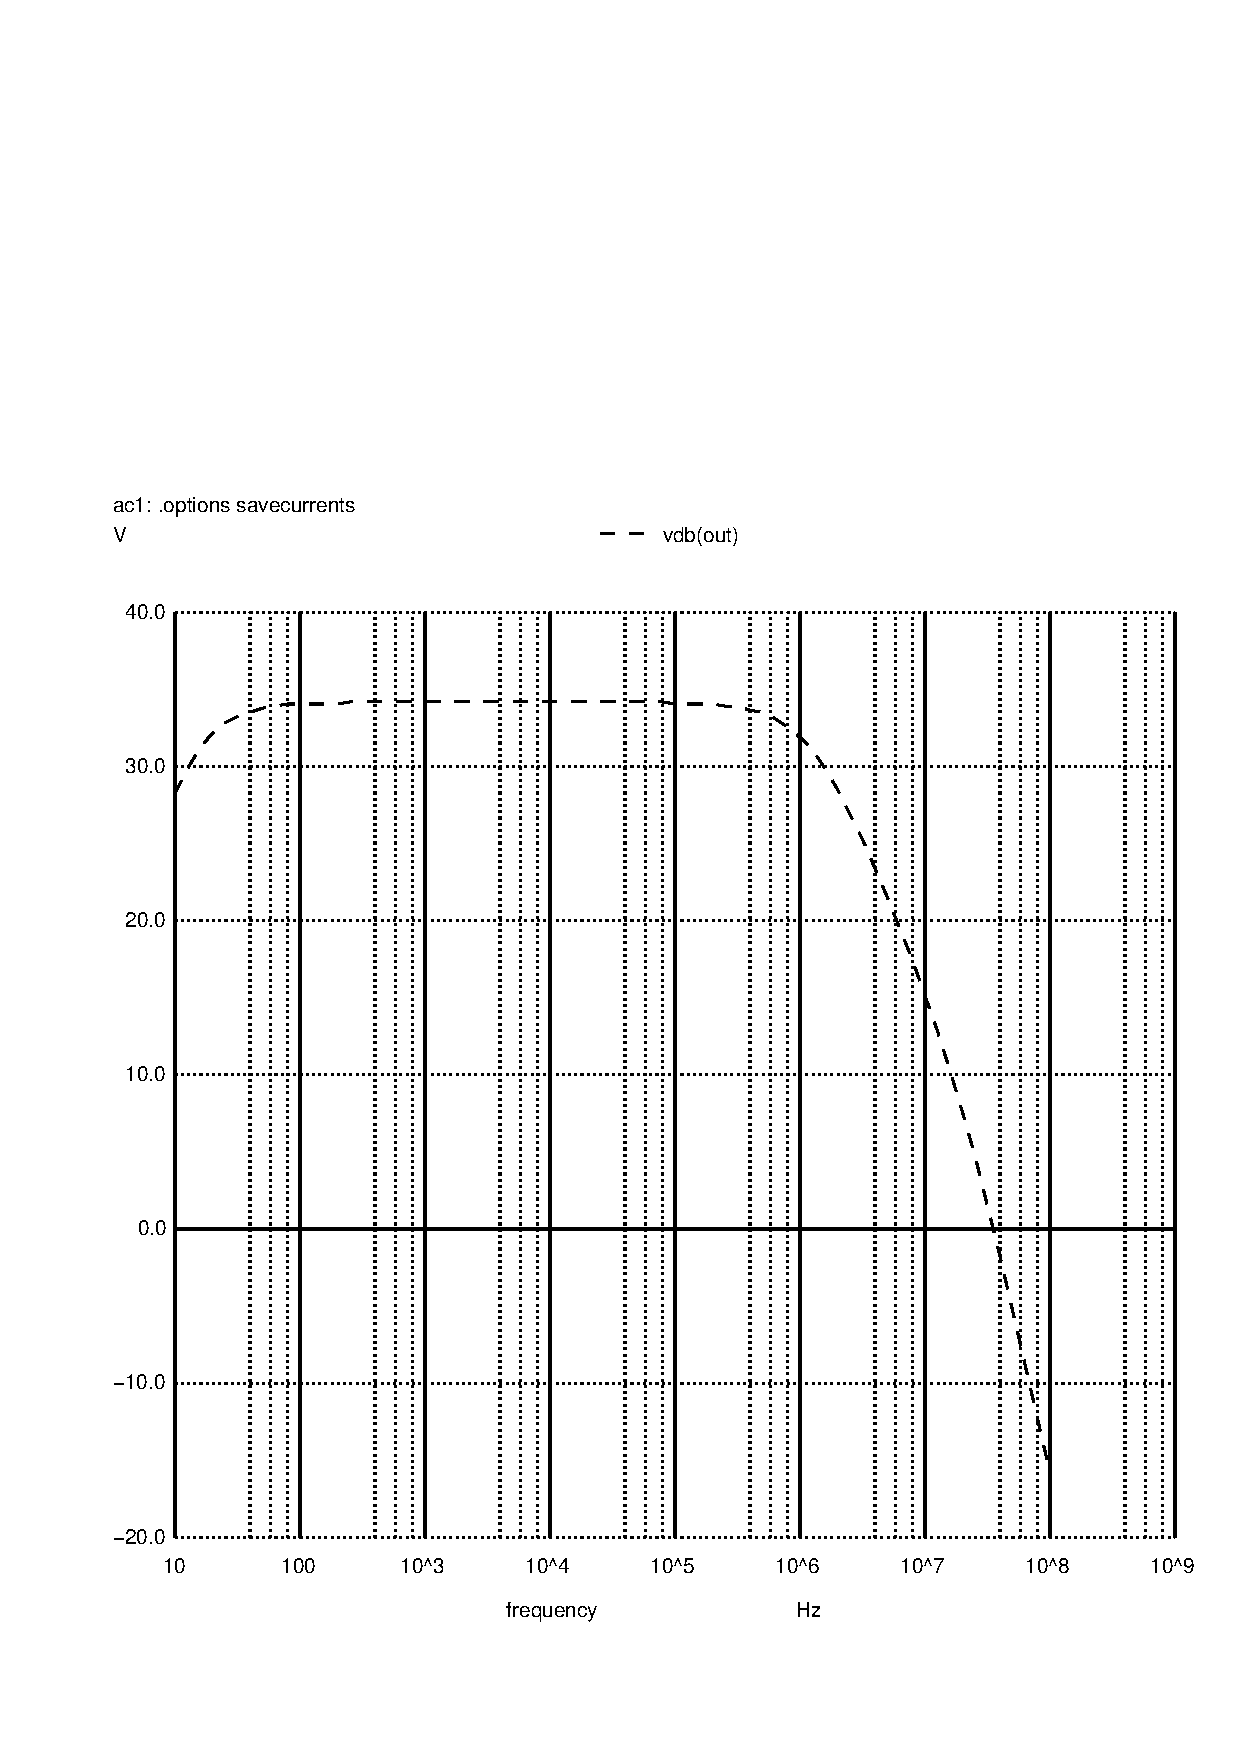
\includegraphics[width=.75\linewidth]{vo2f.pdf}
  \caption{Output voltage}
  \label{fig:sim5}
\end{subfigure}
\end{figure}


\par Next, the input and output impedances were calculated as seen on the tables below,

\begin{table}[h]
  \centering
  \begin{tabular}{|l|r|}
    \hline    
   Zin & -1445.61 + 303.661 j\\ \hline

   \end{tabular}
  \caption{Input impedance ($\Omega$)}
    \label{tab:ZI}
\end{table}

\begin{table}[h]
  \centering
  \begin{tabular}{|l|r|}
    \hline    
   Zo & 25.852 + 1.292 j\\ \hline
Zo(int) & 25.8843\\ \hline

   \end{tabular}
  \caption{Output impedance ($\Omega$)}
  
  \label{tab:ZO}
\end{table}

\par As we can see, the input impedance is higher than the outup impedance. This plays well to maximise the gain as the voltage in node in2 needs to be as close to Vin as possible, reducing the losses. To do that, as we can see in the voltage divider formulae, it's necessary to increase the resistance value. The opposite logic is used to the output impedance. Again, considering the voltage divider formulae, the output impedance must be as small as possible to guarantee the maximum output voltage and gain. Even though the output impedance should be lower than the $8\Omega$ to maximise the output voltage, because of the different parameters in the merit formula, our otimization made the value higher than the optimal value if it was the only one. 

\par Finally the cost and merit of the circuit described and seen in the images before  is calculated in ngspice. The results are shown on the table as it follows.

\begin{table}[ht]
  \centering
  \begin{tabular}{|l|r|}
    \hline    
   V Gain&34.1403\\ \hline
Low Cut Off Freq& 15.8089 Hz\\ \hline
High Cut Off Freq& 1.22341E+06 Hz\\ \hline
Bandwidth&1.22339E+06 Hz\\ \hline
Cost & 2198.94 MU\\ \hline
merit & 1201.48\\ \hline

   \end{tabular}
  \caption{Cost and Merit of the circuit}
  \label{tab:cost}
\end{table}

